\documentclass[titlepage]{article}
\usepackage{pgfplots}
\usepackage[unicode, hidelinks]{hyperref}
\usepackage[left=3cm, right=3cm, top=3cm, bottom=3cm]{geometry} % Margins
\usepackage{amsfonts}

\begin{document}

\section*{Stuve diagram in \LaTeX}

\subsection*{Dry adiabats calculation}
\subsubsection*{Diagram}

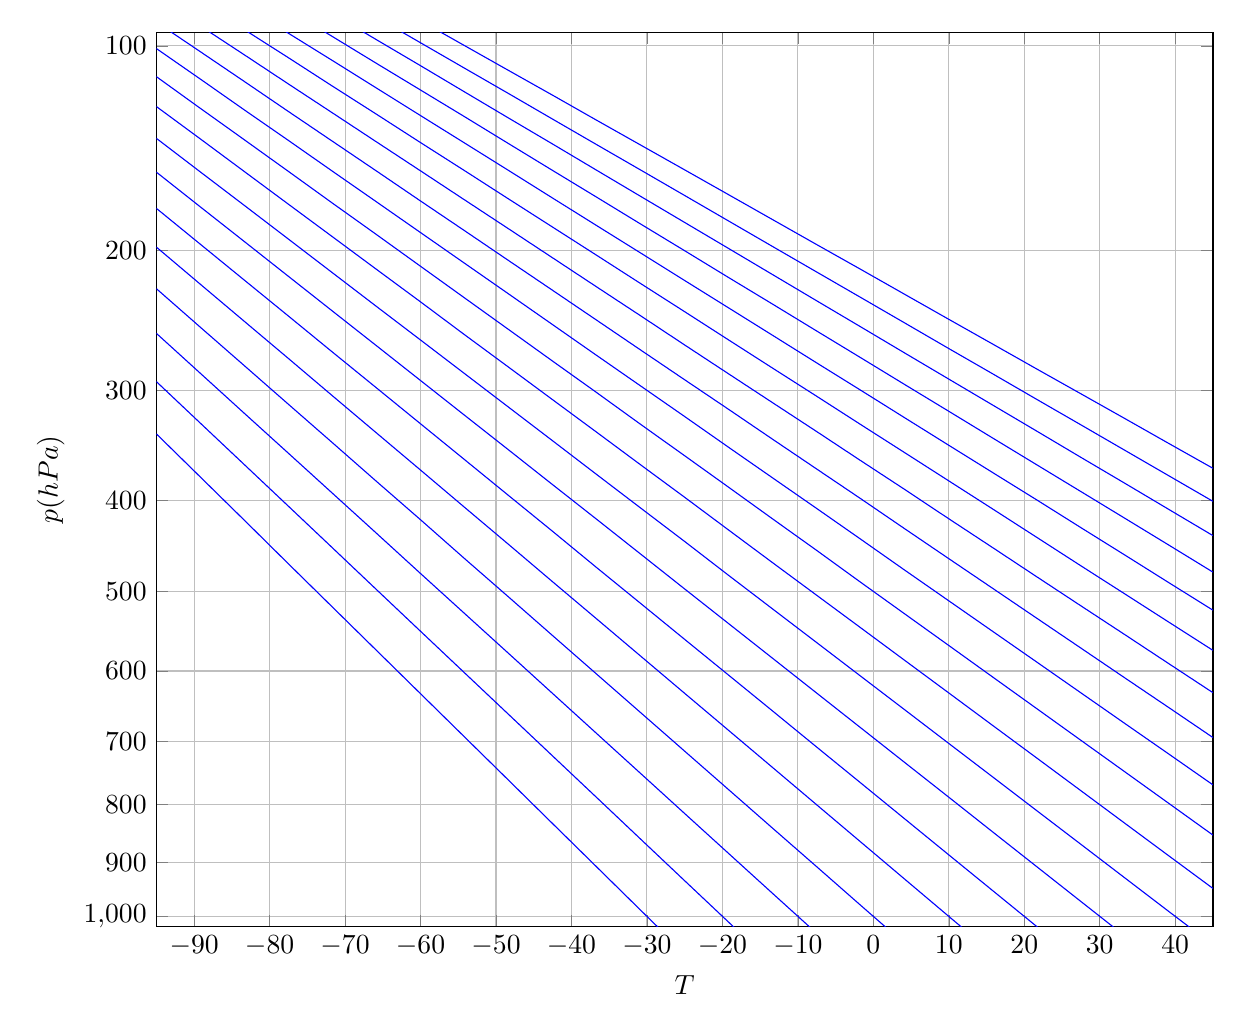
\begin{tikzpicture}
  \begin{axis}[
      xmin=-95,
      xmax=45,
      ymin=95,
      ymax=1020,
      y dir=reverse,
      ytick={100,200,...,1000},
      yticklabel style={/pgf/number format/.cd, precision=0, relative*=2},
      xlabel=\( T \),
      ylabel=\( p (hPa) \),
      grid=both,
      width=15cm,
      y coord trafo/.code={\pgfmathparse{#1^0.286}},
      y coord inv trafo/.code={\pgfmathparse{#1^(1/0.286)}},
    ]
    \foreach \T in {-30,-20,..., 150} {
        \addplot [blue, domain=-95:45] {1000*((x + 273.15)/(\T + 273.15))^(1/0.286)};
      };
  \end{axis}
\end{tikzpicture}
\subsubsection*{Explanation}

Given the following dry adiabats formula\footnote{\href{https://www.eoas.ubc.ca/books/Practical\_Meteorology/}{Stull, Roland: \textit{Practical Meteorology: An Algebra-based Survey of Atmospheric Science}}, chapter 3, p. 61, equation 3.12, 2018} \footnote{\href{https://www.igf.fuw.edu.pl/m/courses\_materials/7c/dd/7cdd179d-d7dc-44dc-9394-dfab086cb84a/thermodynamic\_diagrams.pdf}{www.igf.fuw.edu.pl/m/courses\_materials.../thermodynamic\_diagrams.pdf}}:

\[ \phi = T \cdot \biggl(\frac{p_0}{p}\biggr)^k \]

We know that \( \phi \) refers to the \( x \) axis, and \( p \) to the \( y \) axis, so we can rearrange to solve for \( p \):

\[ \frac{\phi}{T} = \biggl(\frac{p_0}{p}\biggr)^{k} \]
\[ \biggl(\frac{\phi}{T}\biggr)^{\frac{1}{k}} = \frac{p_0}{p} \]
\[ \biggl(\frac{T}{\phi}\biggr)^{\frac{1}{k}} = \frac{p}{p_0} \]
\[ p_0 \cdot \biggl(\frac{T}{\phi}\biggr)^{\frac{1}{k}} = p \]
\[ p = p_0 \cdot \biggl(\frac{T}{\phi}\biggr)^{\frac{1}{k}} \]

We know that \( \phi \) refers to the \( x \) axis, and \( p \) to the \( y \) axis, while \( p_0 \) is the initial pressure with a standart value of 1000 hPa, and \( k \) the Poisson constant, the ratio of the gas constant to the specific heat capacity at constant pressure for an ideal diatomic gas\footnote{See \href{resources.eumetrain.org/data/2/28/Content/theta.htm}{https://resources.eumetrain.org/data/2/28/Content/theta.htm}}.

\[ \phi = x ; \quad p = y ; \quad p_0 = 1000 ; \quad k = 0.286 \]

We can replace variables:

\[ y = 1000 \cdot \biggl(\frac{T}{x}\biggr)^{\frac{1}{0.286}} \]

And knowing that temperature should be in Kelvin:

\[ y = 1000 \cdot \biggl(\frac{T + 273.15}{x + 273.15}\biggr)^{\frac{1}{0.286}} \]
Which gives us a formula to use in the LaTeX diagram.

\begin{verbatim}
    1000 * ((x + 273.15) / (\T + 273.15))^(1/0.286)
\end{verbatim}

Also, we shoult take into account that in Stuve diagrams we want to draw the dry adiabats as straight lines. Thus \( y \) axis is not logarithmic, but progressing in a ratio of \( y^{k} \), or \( y^{0.286} \).

\begin{verbatim}
  \begin{axis}[
    [...]
    y coord trafo/.code={\pgfmathparse{#1^0.286}},
    y coord inv trafo/.code={\pgfmathparse{#1^(1/0.286)}},
  ]
\end{verbatim}

\vspace*{\fill}

\subsection*{Isohumes calculation (Work in Progress)}
\subsubsection*{Diagram}
\subsubsection*{First try}

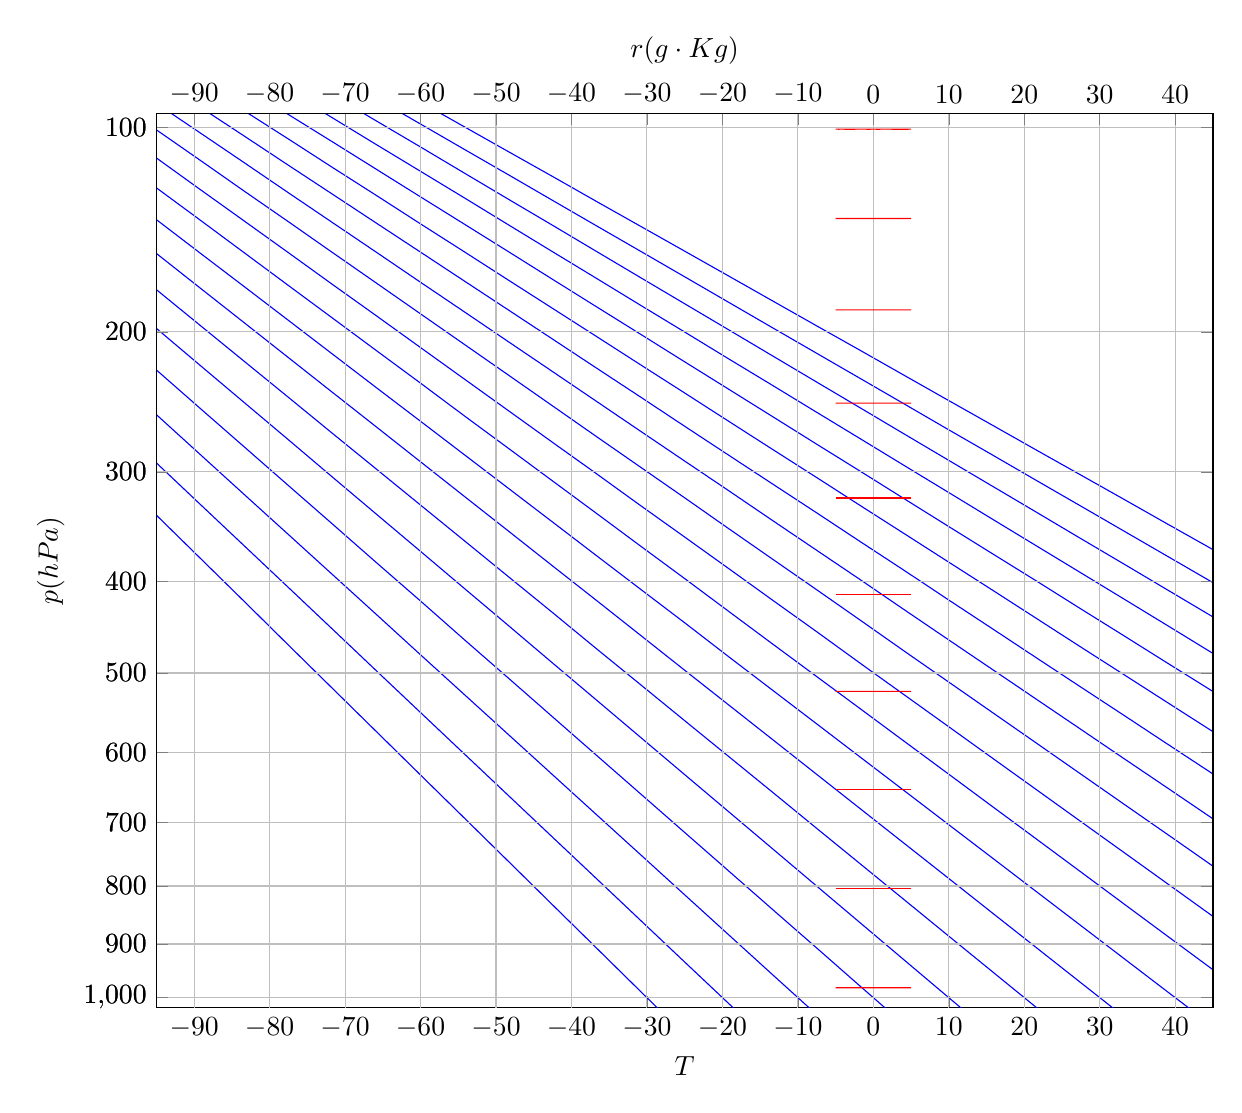
\begin{tikzpicture}
  \begin{axis}[
      xmin=-95,
      xmax=45,
      ymin=95,
      ymax=1020,
      y dir=reverse,
      ytick={100,200,...,1000},
      yticklabel style={/pgf/number format/.cd, precision=0, relative*=2},
      xlabel=\( T \),
      ylabel=\( p (hPa) \),
      grid=both,
      width=15cm,
      y coord trafo/.code={\pgfmathparse{#1^0.286}},
      y coord inv trafo/.code={\pgfmathparse{#1^(1/0.286)}},
    ]
    \foreach \T in {-30,-20,..., 150} {
        \addplot [blue, domain=-95:45] {1000*((x + 273.15)/(\T + 273.15))^(1/0.286)};
      };
  \end{axis}
  \begin{axis}[
      xmin=-95,
      xmax=45,
      ymin=95,
      ymax=1020,
      y dir=reverse,
      ytick={100,200,...,1000},
      yticklabel style={/pgf/number format/.cd, precision=0, relative*=2},
      xlabel=\( r (g \cdot Kg) \),
      xlabel near ticks,
      grid=both,
      width=15cm,
      y coord trafo/.code={\pgfmathparse{#1^0.286}},
      y coord inv trafo/.code={\pgfmathparse{#1^(1/0.286)}},
      axis x line*=top
    ]
    \foreach \T in {-30,-20,..., 150} {
        \addplot [red] {((0.23620100952 * exp((12.27 * \T)/(237.3 + \T))) + (x * 0.61078 * exp((12.27 * \T)/(237.3 + \T))) / x) * 10};
      };
  \end{axis}
\end{tikzpicture}

\subsubsection*{Explanation}

Given the following formula\footnote{See \href{https://www.igf.fuw.edu.pl/m/courses\_materials/7c/dd/7cdd179d-d7dc-44dc-9394-dfab086cb84a/thermodynamic\_diagrams.pdf}{www.igf.fuw.edu.pl/m/courses\_materials.../thermodynamic\_diagrams.pdf}}:

\[ r_s = \varepsilon \cdot \frac{e_s(T)}{p - e_s(T)} \]

% And asuming that \( e_s \) is the Tetens equation\footnote{See \href{https://en.wikipedia.org/wiki/Tetens_equation/}{https://en.wikipedia.org/wiki/Tetens_equation}}:
And asuming that \( e_s(T) \) is the Tetens equation\footnote{See \href{https://en.wikipedia.org/wiki/Tetens\_equation}{en.wikipedia.org/wiki/Tetens\_equation}}:

\[ e_s(T) = 0.61078 \cdot \exp \biggl(\frac{12.27 \cdot T}{237.3 + T}\biggr) \]

We know that \( r_s \) refers to the \( x \) axis, and \( p \) to the \( y \) axis.
\[ r_s = x ; \quad p = y \]

\[ x = \varepsilon \cdot \frac{e_s(T)}{y - e_s(T)} \]

Then we can solve for \( y \):

\[ x = \frac{\varepsilon \cdot e_s(T)}{y - e_s(T)} \]

\[ y - e_s(T) = \frac{\varepsilon \cdot e_s(T)}{x} \]

\[ y  = \frac{\varepsilon \cdot e_s(T)}{x} + e_s(T) \]

\[ y  = \frac{(\varepsilon \cdot e_s(T)) + (x \cdot e_s(T))}{x} \]

\[ y  = \frac{(\varepsilon \cdot 0.61078 \cdot \exp(\frac{12.27 \cdot T}{237.3 + T})) + (x \cdot 0.61078 \cdot \exp(\frac{12.27 \cdot T}{237.3 + T}))}{x} \]

We also know that \( \varepsilon \) is a constant: the ratio between the gas constant for dry air and the gas constant for water vapor\footnote{See \href{https://pressbooks-dev.oer.hawaii.edu/atmo/chapter/chapter-4-water-vapor/}{pressbooks-dev.oer.hawaii.edu/atmo/chapter/chapter-4-water-vapor/}}:

\[ \varepsilon = 0.622 \]

We replace \( \varepsilon \):

\[ y  = \frac{(0.622 \cdot 0.61078 \cdot \exp(\frac{12.27 \cdot T}{237.3 + T})) + (x \cdot 0.61078 \cdot \exp(\frac{12.27 \cdot T}{237.3 + T}))}{x} \]

\[ y  = \frac{(0.23620100952 \cdot \exp(\frac{12.27 \cdot T}{237.3 + T})) + (x \cdot 0.61078 \cdot \exp(\frac{12.27 \cdot T}{237.3 + T}))}{x} \]


Which we should be able to use in LaTeX:

\begin{verbatim}
  ((0.23620100952 * exp((12.27 * \T)/(237.3 + \T))) + (x * 0.61078 * exp((12.27 * \T)/(237.3 + \T))) / x) * 10
\end{verbatim}

\textcolor{red}{\sc{NOT RENDERING PROPER HISOHUMES}}

\vspace*{\fill}

\subsubsection*{Second try}

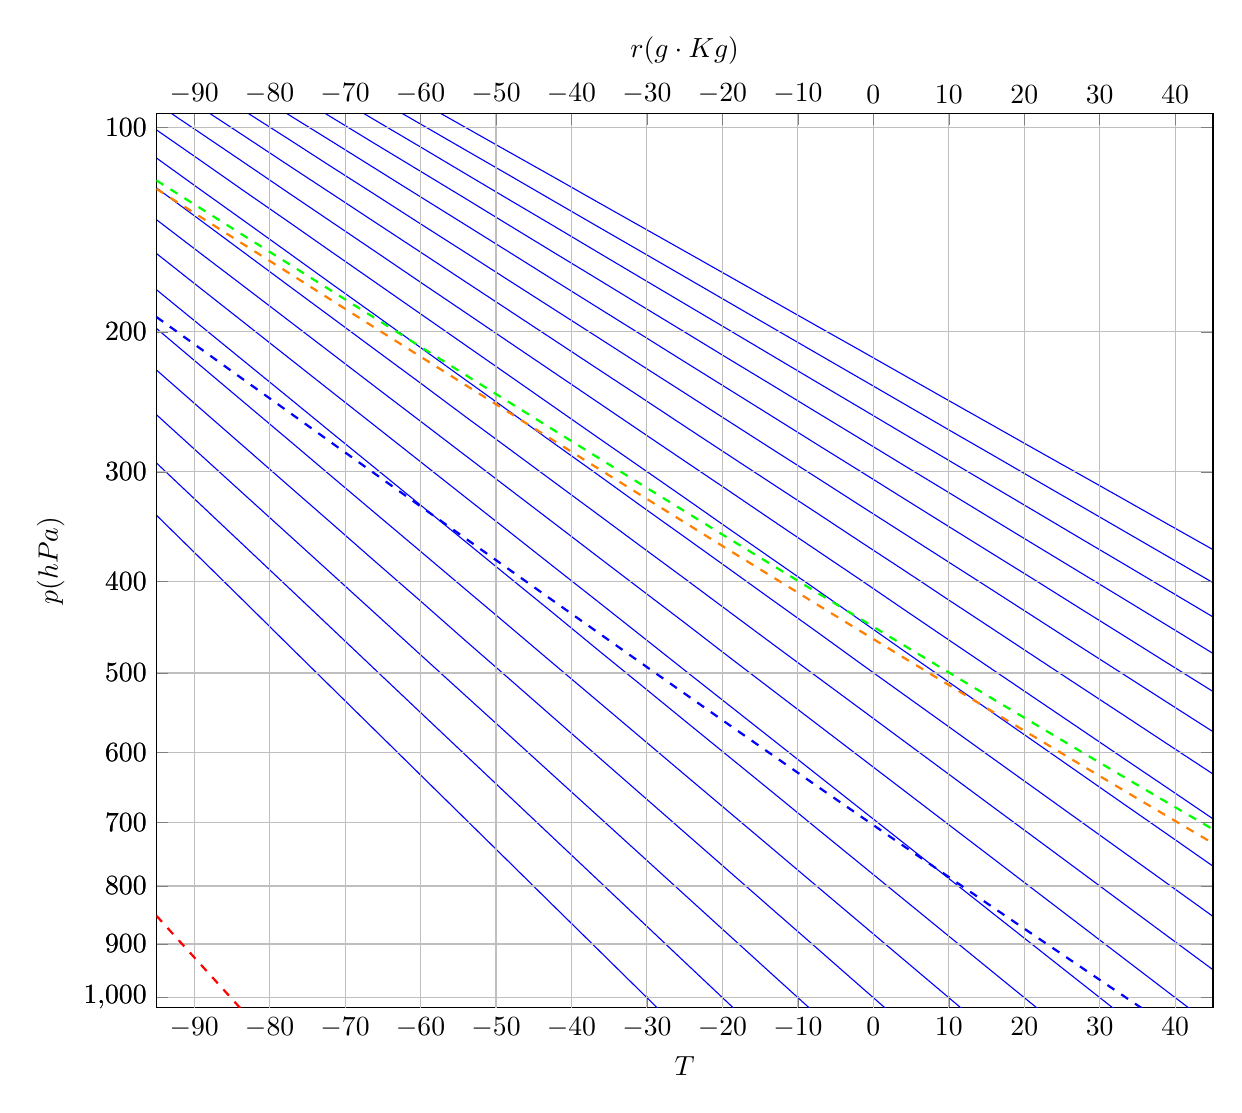
\begin{tikzpicture}
  \begin{axis}[
      xmin=-95,
      xmax=45,
      ymin=95,
      ymax=1020,
      y dir=reverse,
      ytick={100,200,...,1000},
      yticklabel style={/pgf/number format/.cd, precision=0, relative*=2},
      xlabel=\( T \),
      ylabel=\( p (hPa) \),
      grid=both,
      width=15cm,
      y coord trafo/.code={\pgfmathparse{#1^0.286}},
      y coord inv trafo/.code={\pgfmathparse{#1^(1/0.286)}},
    ]
    \foreach \T in {-30,-20,..., 150} {
        \addplot [blue, domain=-95:45] {1000*((x + 273.15)/(\T + 273.15))^(1/0.286)};
      };
  \end{axis}
  \begin{axis}[
      xmin=-95,
      xmax=45,
      ymin=95,
      ymax=1020,
      y dir=reverse,
      ytick={100,200,...,1000},
      yticklabel style={/pgf/number format/.cd, precision=0, relative*=2},
      xlabel=\( r (g \cdot Kg) \),
      xlabel near ticks,
      grid=both,
      width=15cm,
      y coord trafo/.code={\pgfmathparse{#1^0.286}},
      y coord inv trafo/.code={\pgfmathparse{#1^(1/0.286)}},
      axis x line*=top
    ]
    \addplot [red, dashed, thick, domain=-95:45] {( 0.622 * 0.61078 * exp( ( 12.27 * (x + 273.15) ) / ( 237.3 + (x + 273.15) )) + (0.1 * 0.61078 *  exp( ( 12.27 * (x + 273.15) ) / ( 237.3 + (x + 273.15) )) )) / ( 0.1 )};
    \addplot [blue, dashed, thick, domain=-95:45] {( 0.622 * 0.61078 * exp( ( 12.27 * (x + 273.15) ) / ( 237.3 + (x + 273.15) )) + (1 * 0.61078 *  exp( ( 12.27 * (x + 273.15) ) / ( 237.3 + (x + 273.15) )) )) / ( 1 )};
    \addplot [orange, dashed, thick, domain=-95:45] {( 0.622 * 0.61078 * exp( ( 12.27 * (x + 273.15) ) / ( 237.3 + (x + 273.15) )) + (10 * 0.61078 *  exp( ( 12.27 * (x + 273.15) ) / ( 237.3 + (x + 273.15) )) )) / ( 10 )};
    \addplot [green, dashed, thick, domain=-95:45] {( 0.622 * 0.61078 * exp( ( 12.27 * (x + 273.15) ) / ( 237.3 + (x + 273.15) )) + (20 * 0.61078 *  exp( ( 12.27 * (x + 273.15) ) / ( 237.3 + (x + 273.15) )) )) / ( 20 )};
  \end{axis}
\end{tikzpicture}

\subsubsection*{Explanation}

Given the following formula\footnote{See \href{https://www.igf.fuw.edu.pl/m/courses\_materials/7c/dd/7cdd179d-d7dc-44dc-9394-dfab086cb84a/thermodynamic\_diagrams.pdf}{www.igf.fuw.edu.pl/m/courses\_materials.../thermodynamic\_diagrams.pdf}}:

\[ r_s = \frac{\varepsilon \cdot e_s(T)}{p - e_s(T)} \]

% And asuming that \( e_s \) is the Tetens equation\footnote{See \href{https://en.wikipedia.org/wiki/Tetens_equation/}{https://en.wikipedia.org/wiki/Tetens_equation}}:
And asuming that \( e_s(T) \) is the Tetens equation\footnote{See \href{https://en.wikipedia.org/wiki/Tetens\_equation}{en.wikipedia.org/wiki/Tetens\_equation}}:

\[ e_s(T) = 0.61078 \cdot \exp \biggl(\frac{12.27 \cdot T}{237.3 + T}\biggr) \]

We know that \( T \) refers to the \( x \) axis, and \( p \) to the \( y \) axis.
\[ T = x ; \quad p = y \]

\[ r_s =\frac{\varepsilon \cdot 0.61078 \cdot \exp \bigl(\frac{12.27 \cdot T}{237.3 + T}\bigr)}{p - \biggl( 0.61078 \cdot \exp \bigl(\frac{12.27 \cdot T}{237.3 + T}\bigr)\biggr)} \]

We can solve for \( p \):

\[ r_s \cdot \Biggl( p - \biggl( 0.61078 \cdot \exp \bigl(\frac{12.27 \cdot T}{237.3 + T}\bigr)\biggr)\Biggr) = \varepsilon \cdot 0.61078 \cdot \exp \biggl(\frac{12.27 \cdot T}{237.3 + T}\biggr) \]

\[ p - \biggl( 0.61078 \cdot \exp \bigl(\frac{12.27 \cdot T}{237.3 + T}\bigr)\biggr) = \frac{\varepsilon \cdot 0.61078 \cdot \exp \biggl(\frac{12.27 \cdot T}{237.3 + T}\biggr)}{r_s} \]

\[ p  = \frac{\varepsilon \cdot 0.61078 \cdot \exp \biggl(\frac{12.27 \cdot T}{237.3 + T}\biggr)}{r_s} + \biggl( 0.61078 \cdot \exp \bigl(\frac{12.27 \cdot T}{237.3 + T}\bigr)\biggr)\]

\[ p  = \frac{\biggl(\varepsilon \cdot 0.61078 \cdot \exp \biggl(\frac{12.27 \cdot T}{237.3 + T}\biggr)\biggr) + \biggl( r_s \cdot 0.61078 \cdot \exp \bigl(\frac{12.27 \cdot T}{237.3 + T} \bigr)\biggr) }{r_s} \]

\[ \varepsilon = 0.622 \]

\[ p  = \frac{\biggl(0.622 \cdot 0.61078 \cdot \exp \biggl(\frac{12.27 \cdot T}{237.3 + T}\biggr)\biggr) + \biggl( r_s \cdot 0.61078 \cdot \exp \bigl(\frac{12.27 \cdot T}{237.3 + T} \bigr)\biggr) }{r_s} \]

Which we should be able to use in LaTeX:

\begin{verbatim}
  ( 0.622 * 0.61078 * exp( ( 12.27 * x ) / ( 237.3 + x )) + (r_s * 0.61078 *  exp( ( 12.27 * x ) / ( 237.3 + x )) )) / ( r_s )
\end{verbatim}


\begin{verbatim}

\end{verbatim}

\textcolor{red}{\sc{NOT RENDERING PROPER HISOHUMES}}

\vspace*{\fill}

\subsubsection*{Third try}

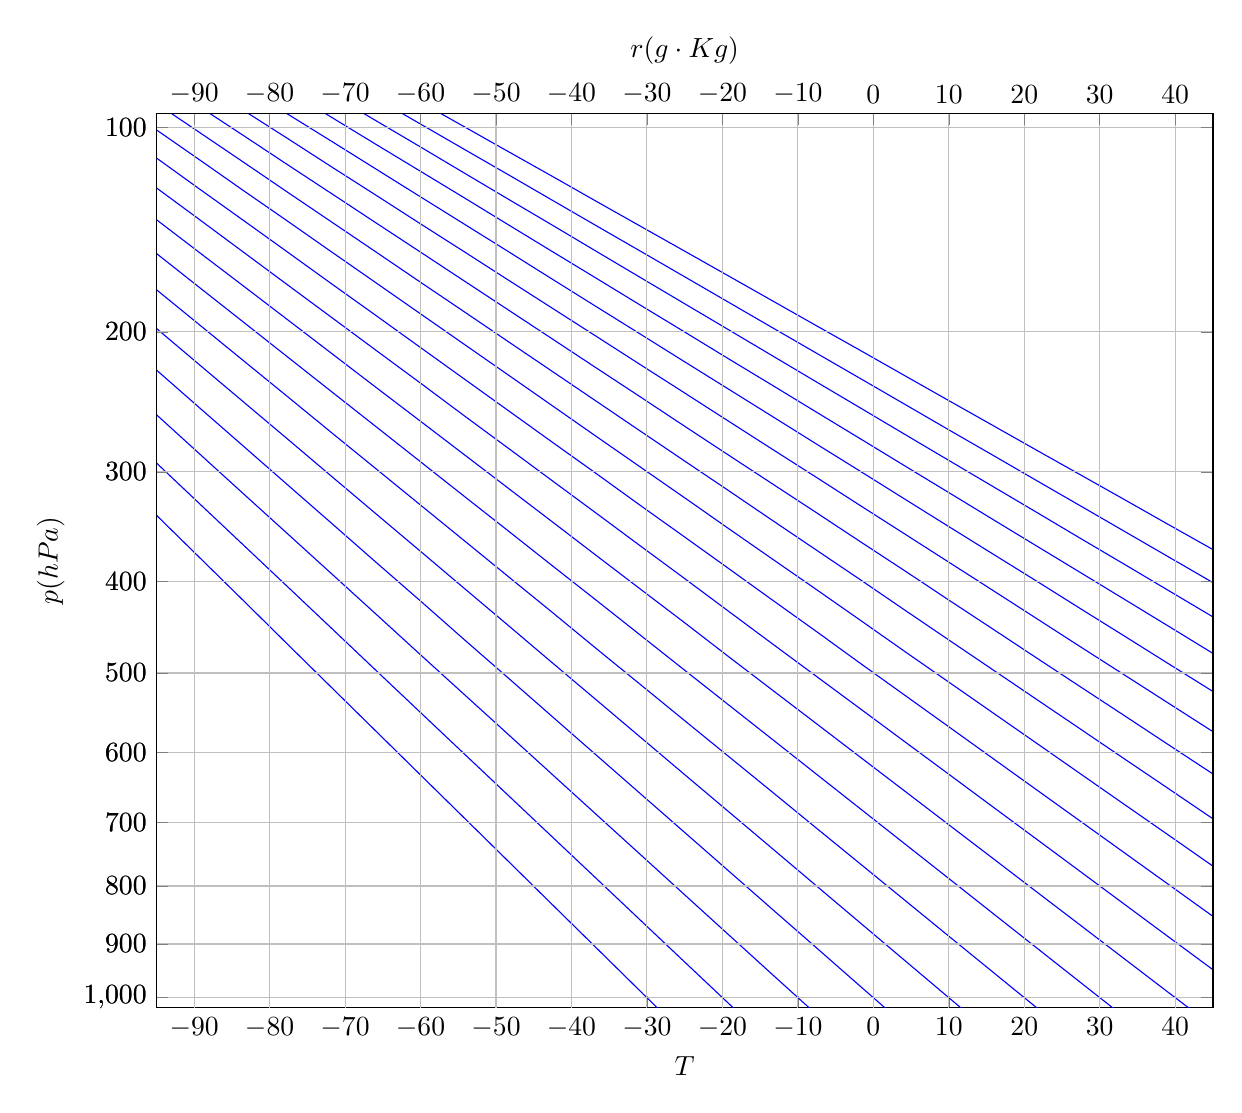
\begin{tikzpicture}
  \begin{axis}[
      xmin=-95,
      xmax=45,
      ymin=95,
      ymax=1020,
      y dir=reverse,
      ytick={100,200,...,1000},
      yticklabel style={/pgf/number format/.cd, precision=0, relative*=2},
      xlabel=\( T \),
      ylabel=\( p (hPa) \),
      grid=both,
      width=15cm,
      y coord trafo/.code={\pgfmathparse{#1^0.286}},
      y coord inv trafo/.code={\pgfmathparse{#1^(1/0.286)}},
    ]
    \foreach \T in {-30,-20,..., 150} {
        \addplot [blue, domain=-95:45] {1000*((x + 273.15)/(\T + 273.15))^(1/0.286)};
      };
  \end{axis}
  \begin{axis}[
      xmin=-95,
      xmax=45,
      ymin=95,
      ymax=1020,
      y dir=reverse,
      ytick={100,200,...,1000},
      yticklabel style={/pgf/number format/.cd, precision=0, relative*=2},
      xlabel=\( r (g \cdot Kg) \),
      xlabel near ticks,
      grid=both,
      width=15cm,
      y coord trafo/.code={\pgfmathparse{#1^0.286}},
      y coord inv trafo/.code={\pgfmathparse{#1^(1/0.286)}},
      axis x line*=top
    ]

    \addplot [blue, dashed, domain=-95:45] { (exp(((x + 273.15) - 273.15) / ((x + 273.15) * 273.15 * 0.0001844)) * 0.6113 * (1 + 0.622 ) ) /1 };
    \addplot [red,dashed, domain=-95:45] { (exp(((x + 273.15) - 273.15) / ((x + 273.15) * 273.15 * 0.0001844)) * 0.6113 * ( 1 + 0.622 ) ) / 1 };
  \end{axis}
\end{tikzpicture}

\subsubsection*{Explanation}

Following the equation found on \textit{Practical Meteorology: An Algebra-based Survey of Atmospheric Science}:\footnote{\href{https://www.eoas.ubc.ca/books/Practical\_Meteorology/}{Stull, Roland: \textit{Practical Meteorology: An Algebra-based Survey of Atmospheric Science}}, chapter 4, p. 101, equation 4.36, 2018}
\[ T = \biggl[ \frac{1}{T_0} - \frac{\mathfrak{R}_v}{L_v} \cdot \ln\biggl(\frac{r_s \cdot p}{e_0 \cdot (r_s + \varepsilon)}\biggr)  \biggr]^{-1} \]

We should be able to solve for  \( p \):

\[ \frac{1}{T} = \frac{1}{T_0} - \frac{\mathfrak{R}_v}{L_v} \cdot \ln\biggl(\frac{r_s \cdot p}{e_0 \cdot (r_s + \varepsilon)}\biggr) \]

\[  \frac{1}{T} + \frac{\mathfrak{R}_v}{L_v} \cdot \ln\biggl(\frac{r_s \cdot p}{e_0 \cdot (r_s + \varepsilon)}\biggr) = \frac{1}{T_0} \]

\[ \frac{\mathfrak{R}_v}{L_v} \cdot \ln\biggl(\frac{r_s \cdot p}{e_0 \cdot (r_s + \varepsilon)}\biggr) = \frac{1}{T_0} - \frac{1}{T} \]

\[ \frac{\mathfrak{R}_v}{L_v} \cdot \ln\biggl(\frac{r_s \cdot p}{e_0 \cdot (r_s + \varepsilon)}\biggr) = \frac{T - T_0}{T \cdot T_0} \]

\[ \ln\biggl(\frac{r_s \cdot p}{e_0 \cdot (r_s + \varepsilon)}\biggr) = \frac{T - T_0}{T \cdot T_0 \cdot \frac{\mathfrak{R}_v}{L_v}} \]

\[ \frac{r_s \cdot p}{e_0 \cdot (r_s + \varepsilon)} = exp\biggl(\frac{T - T_0}{T \cdot T_0 \cdot \frac{\mathfrak{R}_v}{L_v}}\biggr) \]

\[ r_s \cdot p = exp\biggl(\frac{T - T_0}{T \cdot T_0 \cdot \frac{\mathfrak{R}_v}{L_v}}\biggr) \cdot e_0 \cdot (r_s + \varepsilon) \]

\[ p = \frac{exp\biggl(\frac{T - T_0}{T \cdot T_0 \cdot \frac{\mathfrak{R}_v}{L_v}}\biggr) \cdot e_0 \cdot (r_s + \varepsilon)}{r_s} \]


\[ T_0 = 273.15 \qquad e_0 = 0.6113 \qquad \frac{\mathfrak{R}_v}{L_v} = 0.0001844 \qquad \varepsilon = 0.622 \]

\[ p = \frac{exp\biggl(\frac{T - 273.15}{T \cdot 273.15 \cdot 0.0001844}\biggr) \cdot 0.6113 \cdot (r_s + 0.622)}{r_s} \]

\[ T = x \qquad p = y \]

\[ p = \frac{exp\biggl(\frac{x - 273.15}{x \cdot 273.15 \cdot 0.0001844}\biggr) \cdot 0.6113 \cdot (r_s + 0.622)}{r_s} \]

\textcolor{red}{\sc{NOT RENDERING PROPER HISOHUMES}}


\vspace*{\fill}

\end{document}
